\documentclass[11pt]{article}

    \usepackage[breakable]{tcolorbox}
    \usepackage{parskip} % Stop auto-indenting (to mimic markdown behaviour)
    
    \usepackage{iftex}
    \ifPDFTeX
    	\usepackage[T1]{fontenc}
    	\usepackage{mathpazo}
    \else
    	\usepackage{fontspec}
    \fi

    % Basic figure setup, for now with no caption control since it's done
    % automatically by Pandoc (which extracts ![](path) syntax from Markdown).
    \usepackage{graphicx}
    % Maintain compatibility with old templates. Remove in nbconvert 6.0
    \let\Oldincludegraphics\includegraphics
    % Ensure that by default, figures have no caption (until we provide a
    % proper Figure object with a Caption API and a way to capture that
    % in the conversion process - todo).
    \usepackage[font=scriptsize]{caption}
    % \DeclareCaptionFormat{nocaption}{}
    % \captionsetup{format=nocaption,aboveskip=0pt,belowskip=0pt}

    \usepackage[Export]{adjustbox} % Used to constrain images to a maximum size
    \adjustboxset{max size={0.9\linewidth}{0.9\paperheight}}
    \usepackage{float}
    \floatplacement{figure}{H} % forces figures to be placed at the correct location
    \usepackage{xcolor} % Allow colors to be defined
    \usepackage{enumerate} % Needed for markdown enumerations to work
    \usepackage{geometry} % Used to adjust the document margins
    \usepackage{amsmath} % Equations
    \usepackage{amssymb} % Equations
    \usepackage{textcomp} % defines textquotesingle
    % Hack from http://tex.stackexchange.com/a/47451/13684:
    \AtBeginDocument{%
        \def\PYZsq{\textquotesingle}% Upright quotes in Pygmentized code
    }
    \usepackage{upquote} % Upright quotes for verbatim code
    \usepackage{eurosym} % defines \euro
    \usepackage[mathletters]{ucs} % Extended unicode (utf-8) support
    \usepackage{fancyvrb} % verbatim replacement that allows latex
    \usepackage{grffile} % extends the file name processing of package graphics 
                         % to support a larger range
    \makeatletter % fix for grffile with XeLaTeX
    \def\Gread@@xetex#1{%
      \IfFileExists{"\Gin@base".bb}%
      {\Gread@eps{\Gin@base.bb}}%
      {\Gread@@xetex@aux#1}%
    }
    \makeatother

    % The hyperref package gives us a pdf with properly built
    % internal navigation ('pdf bookmarks' for the table of contents,
    % internal cross-reference links, web links for URLs, etc.)
    \usepackage{hyperref}
    % The default LaTeX title has an obnoxious amount of whitespace. By default,
    % titling removes some of it. It also provides customization options.
    \usepackage{titling}
    \usepackage{longtable} % longtable support required by pandoc >1.10
    \usepackage{booktabs}  % table support for pandoc > 1.12.2
    \usepackage[inline]{enumitem} % IRkernel/repr support (it uses the enumerate* environment)
    \usepackage[normalem]{ulem} % ulem is needed to support strikethroughs (\sout)
                                % normalem makes italics be italics, not underlines
    \usepackage{mathrsfs}
    

    
    % Colors for the hyperref package
    \definecolor{urlcolor}{rgb}{0,.145,.698}
    \definecolor{linkcolor}{rgb}{.71,0.21,0.01}
    \definecolor{citecolor}{rgb}{.12,.54,.11}

    % ANSI colors
    \definecolor{ansi-black}{HTML}{3E424D}
    \definecolor{ansi-black-intense}{HTML}{282C36}
    \definecolor{ansi-red}{HTML}{E75C58}
    \definecolor{ansi-red-intense}{HTML}{B22B31}
    \definecolor{ansi-green}{HTML}{00A250}
    \definecolor{ansi-green-intense}{HTML}{007427}
    \definecolor{ansi-yellow}{HTML}{DDB62B}
    \definecolor{ansi-yellow-intense}{HTML}{B27D12}
    \definecolor{ansi-blue}{HTML}{208FFB}
    \definecolor{ansi-blue-intense}{HTML}{0065CA}
    \definecolor{ansi-magenta}{HTML}{D160C4}
    \definecolor{ansi-magenta-intense}{HTML}{A03196}
    \definecolor{ansi-cyan}{HTML}{60C6C8}
    \definecolor{ansi-cyan-intense}{HTML}{258F8F}
    \definecolor{ansi-white}{HTML}{C5C1B4}
    \definecolor{ansi-white-intense}{HTML}{A1A6B2}
    \definecolor{ansi-default-inverse-fg}{HTML}{FFFFFF}
    \definecolor{ansi-default-inverse-bg}{HTML}{000000}

    % commands and environments needed by pandoc snippets
    % extracted from the output of `pandoc -s`
    \providecommand{\tightlist}{%
      \setlength{\itemsep}{0pt}\setlength{\parskip}{0pt}}
    \DefineVerbatimEnvironment{Highlighting}{Verbatim}{commandchars=\\\{\}}
    % Add ',fontsize=\small' for more characters per line
    \newenvironment{Shaded}{}{}
    \newcommand{\KeywordTok}[1]{\textcolor[rgb]{0.00,0.44,0.13}{\textbf{{#1}}}}
    \newcommand{\DataTypeTok}[1]{\textcolor[rgb]{0.56,0.13,0.00}{{#1}}}
    \newcommand{\DecValTok}[1]{\textcolor[rgb]{0.25,0.63,0.44}{{#1}}}
    \newcommand{\BaseNTok}[1]{\textcolor[rgb]{0.25,0.63,0.44}{{#1}}}
    \newcommand{\FloatTok}[1]{\textcolor[rgb]{0.25,0.63,0.44}{{#1}}}
    \newcommand{\CharTok}[1]{\textcolor[rgb]{0.25,0.44,0.63}{{#1}}}
    \newcommand{\StringTok}[1]{\textcolor[rgb]{0.25,0.44,0.63}{{#1}}}
    \newcommand{\CommentTok}[1]{\textcolor[rgb]{0.38,0.63,0.69}{\textit{{#1}}}}
    \newcommand{\OtherTok}[1]{\textcolor[rgb]{0.00,0.44,0.13}{{#1}}}
    \newcommand{\AlertTok}[1]{\textcolor[rgb]{1.00,0.00,0.00}{\textbf{{#1}}}}
    \newcommand{\FunctionTok}[1]{\textcolor[rgb]{0.02,0.16,0.49}{{#1}}}
    \newcommand{\RegionMarkerTok}[1]{{#1}}
    \newcommand{\ErrorTok}[1]{\textcolor[rgb]{1.00,0.00,0.00}{\textbf{{#1}}}}
    \newcommand{\NormalTok}[1]{{#1}}
    
    % Additional commands for more recent versions of Pandoc
    \newcommand{\ConstantTok}[1]{\textcolor[rgb]{0.53,0.00,0.00}{{#1}}}
    \newcommand{\SpecialCharTok}[1]{\textcolor[rgb]{0.25,0.44,0.63}{{#1}}}
    \newcommand{\VerbatimStringTok}[1]{\textcolor[rgb]{0.25,0.44,0.63}{{#1}}}
    \newcommand{\SpecialStringTok}[1]{\textcolor[rgb]{0.73,0.40,0.53}{{#1}}}
    \newcommand{\ImportTok}[1]{{#1}}
    \newcommand{\DocumentationTok}[1]{\textcolor[rgb]{0.73,0.13,0.13}{\textit{{#1}}}}
    \newcommand{\AnnotationTok}[1]{\textcolor[rgb]{0.38,0.63,0.69}{\textbf{\textit{{#1}}}}}
    \newcommand{\CommentVarTok}[1]{\textcolor[rgb]{0.38,0.63,0.69}{\textbf{\textit{{#1}}}}}
    \newcommand{\VariableTok}[1]{\textcolor[rgb]{0.10,0.09,0.49}{{#1}}}
    \newcommand{\ControlFlowTok}[1]{\textcolor[rgb]{0.00,0.44,0.13}{\textbf{{#1}}}}
    \newcommand{\OperatorTok}[1]{\textcolor[rgb]{0.40,0.40,0.40}{{#1}}}
    \newcommand{\BuiltInTok}[1]{{#1}}
    \newcommand{\ExtensionTok}[1]{{#1}}
    \newcommand{\PreprocessorTok}[1]{\textcolor[rgb]{0.74,0.48,0.00}{{#1}}}
    \newcommand{\AttributeTok}[1]{\textcolor[rgb]{0.49,0.56,0.16}{{#1}}}
    \newcommand{\InformationTok}[1]{\textcolor[rgb]{0.38,0.63,0.69}{\textbf{\textit{{#1}}}}}
    \newcommand{\WarningTok}[1]{\textcolor[rgb]{0.38,0.63,0.69}{\textbf{\textit{{#1}}}}}
    
    
    % Define a nice break command that doesn't care if a line doesn't already
    % exist.
    \def\br{\hspace*{\fill} \\* }
    % Math Jax compatibility definitions
    \def\gt{>}
    \def\lt{<}
    \let\Oldtex\TeX
    \let\Oldlatex\LaTeX
    \renewcommand{\TeX}{\textrm{\Oldtex}}
    \renewcommand{\LaTeX}{\textrm{\Oldlatex}}
    % Document parameters
    % Document title
    
\title{Calcolo del numero di riproduzione effettivo $R_t$ italiano nel tempo con metodo Bayesiano.}

    
    
\author{Max Pierini\thanks{info@maxpierini.it}}

    
% Pygments definitions
\makeatletter
\def\PY@reset{\let\PY@it=\relax \let\PY@bf=\relax%
    \let\PY@ul=\relax \let\PY@tc=\relax%
    \let\PY@bc=\relax \let\PY@ff=\relax}
\def\PY@tok#1{\csname PY@tok@#1\endcsname}
\def\PY@toks#1+{\ifx\relax#1\empty\else%
    \PY@tok{#1}\expandafter\PY@toks\fi}
\def\PY@do#1{\PY@bc{\PY@tc{\PY@ul{%
    \PY@it{\PY@bf{\PY@ff{#1}}}}}}}
\def\PY#1#2{\PY@reset\PY@toks#1+\relax+\PY@do{#2}}

\expandafter\def\csname PY@tok@w\endcsname{\def\PY@tc##1{\textcolor[rgb]{0.73,0.73,0.73}{##1}}}
\expandafter\def\csname PY@tok@c\endcsname{\let\PY@it=\textit\def\PY@tc##1{\textcolor[rgb]{0.25,0.50,0.50}{##1}}}
\expandafter\def\csname PY@tok@cp\endcsname{\def\PY@tc##1{\textcolor[rgb]{0.74,0.48,0.00}{##1}}}
\expandafter\def\csname PY@tok@k\endcsname{\let\PY@bf=\textbf\def\PY@tc##1{\textcolor[rgb]{0.00,0.50,0.00}{##1}}}
\expandafter\def\csname PY@tok@kp\endcsname{\def\PY@tc##1{\textcolor[rgb]{0.00,0.50,0.00}{##1}}}
\expandafter\def\csname PY@tok@kt\endcsname{\def\PY@tc##1{\textcolor[rgb]{0.69,0.00,0.25}{##1}}}
\expandafter\def\csname PY@tok@o\endcsname{\def\PY@tc##1{\textcolor[rgb]{0.40,0.40,0.40}{##1}}}
\expandafter\def\csname PY@tok@ow\endcsname{\let\PY@bf=\textbf\def\PY@tc##1{\textcolor[rgb]{0.67,0.13,1.00}{##1}}}
\expandafter\def\csname PY@tok@nb\endcsname{\def\PY@tc##1{\textcolor[rgb]{0.00,0.50,0.00}{##1}}}
\expandafter\def\csname PY@tok@nf\endcsname{\def\PY@tc##1{\textcolor[rgb]{0.00,0.00,1.00}{##1}}}
\expandafter\def\csname PY@tok@nc\endcsname{\let\PY@bf=\textbf\def\PY@tc##1{\textcolor[rgb]{0.00,0.00,1.00}{##1}}}
\expandafter\def\csname PY@tok@nn\endcsname{\let\PY@bf=\textbf\def\PY@tc##1{\textcolor[rgb]{0.00,0.00,1.00}{##1}}}
\expandafter\def\csname PY@tok@ne\endcsname{\let\PY@bf=\textbf\def\PY@tc##1{\textcolor[rgb]{0.82,0.25,0.23}{##1}}}
\expandafter\def\csname PY@tok@nv\endcsname{\def\PY@tc##1{\textcolor[rgb]{0.10,0.09,0.49}{##1}}}
\expandafter\def\csname PY@tok@no\endcsname{\def\PY@tc##1{\textcolor[rgb]{0.53,0.00,0.00}{##1}}}
\expandafter\def\csname PY@tok@nl\endcsname{\def\PY@tc##1{\textcolor[rgb]{0.63,0.63,0.00}{##1}}}
\expandafter\def\csname PY@tok@ni\endcsname{\let\PY@bf=\textbf\def\PY@tc##1{\textcolor[rgb]{0.60,0.60,0.60}{##1}}}
\expandafter\def\csname PY@tok@na\endcsname{\def\PY@tc##1{\textcolor[rgb]{0.49,0.56,0.16}{##1}}}
\expandafter\def\csname PY@tok@nt\endcsname{\let\PY@bf=\textbf\def\PY@tc##1{\textcolor[rgb]{0.00,0.50,0.00}{##1}}}
\expandafter\def\csname PY@tok@nd\endcsname{\def\PY@tc##1{\textcolor[rgb]{0.67,0.13,1.00}{##1}}}
\expandafter\def\csname PY@tok@s\endcsname{\def\PY@tc##1{\textcolor[rgb]{0.73,0.13,0.13}{##1}}}
\expandafter\def\csname PY@tok@sd\endcsname{\let\PY@it=\textit\def\PY@tc##1{\textcolor[rgb]{0.73,0.13,0.13}{##1}}}
\expandafter\def\csname PY@tok@si\endcsname{\let\PY@bf=\textbf\def\PY@tc##1{\textcolor[rgb]{0.73,0.40,0.53}{##1}}}
\expandafter\def\csname PY@tok@se\endcsname{\let\PY@bf=\textbf\def\PY@tc##1{\textcolor[rgb]{0.73,0.40,0.13}{##1}}}
\expandafter\def\csname PY@tok@sr\endcsname{\def\PY@tc##1{\textcolor[rgb]{0.73,0.40,0.53}{##1}}}
\expandafter\def\csname PY@tok@ss\endcsname{\def\PY@tc##1{\textcolor[rgb]{0.10,0.09,0.49}{##1}}}
\expandafter\def\csname PY@tok@sx\endcsname{\def\PY@tc##1{\textcolor[rgb]{0.00,0.50,0.00}{##1}}}
\expandafter\def\csname PY@tok@m\endcsname{\def\PY@tc##1{\textcolor[rgb]{0.40,0.40,0.40}{##1}}}
\expandafter\def\csname PY@tok@gh\endcsname{\let\PY@bf=\textbf\def\PY@tc##1{\textcolor[rgb]{0.00,0.00,0.50}{##1}}}
\expandafter\def\csname PY@tok@gu\endcsname{\let\PY@bf=\textbf\def\PY@tc##1{\textcolor[rgb]{0.50,0.00,0.50}{##1}}}
\expandafter\def\csname PY@tok@gd\endcsname{\def\PY@tc##1{\textcolor[rgb]{0.63,0.00,0.00}{##1}}}
\expandafter\def\csname PY@tok@gi\endcsname{\def\PY@tc##1{\textcolor[rgb]{0.00,0.63,0.00}{##1}}}
\expandafter\def\csname PY@tok@gr\endcsname{\def\PY@tc##1{\textcolor[rgb]{1.00,0.00,0.00}{##1}}}
\expandafter\def\csname PY@tok@ge\endcsname{\let\PY@it=\textit}
\expandafter\def\csname PY@tok@gs\endcsname{\let\PY@bf=\textbf}
\expandafter\def\csname PY@tok@gp\endcsname{\let\PY@bf=\textbf\def\PY@tc##1{\textcolor[rgb]{0.00,0.00,0.50}{##1}}}
\expandafter\def\csname PY@tok@go\endcsname{\def\PY@tc##1{\textcolor[rgb]{0.53,0.53,0.53}{##1}}}
\expandafter\def\csname PY@tok@gt\endcsname{\def\PY@tc##1{\textcolor[rgb]{0.00,0.27,0.87}{##1}}}
\expandafter\def\csname PY@tok@err\endcsname{\def\PY@bc##1{\setlength{\fboxsep}{0pt}\fcolorbox[rgb]{1.00,0.00,0.00}{1,1,1}{\strut ##1}}}
\expandafter\def\csname PY@tok@kc\endcsname{\let\PY@bf=\textbf\def\PY@tc##1{\textcolor[rgb]{0.00,0.50,0.00}{##1}}}
\expandafter\def\csname PY@tok@kd\endcsname{\let\PY@bf=\textbf\def\PY@tc##1{\textcolor[rgb]{0.00,0.50,0.00}{##1}}}
\expandafter\def\csname PY@tok@kn\endcsname{\let\PY@bf=\textbf\def\PY@tc##1{\textcolor[rgb]{0.00,0.50,0.00}{##1}}}
\expandafter\def\csname PY@tok@kr\endcsname{\let\PY@bf=\textbf\def\PY@tc##1{\textcolor[rgb]{0.00,0.50,0.00}{##1}}}
\expandafter\def\csname PY@tok@bp\endcsname{\def\PY@tc##1{\textcolor[rgb]{0.00,0.50,0.00}{##1}}}
\expandafter\def\csname PY@tok@fm\endcsname{\def\PY@tc##1{\textcolor[rgb]{0.00,0.00,1.00}{##1}}}
\expandafter\def\csname PY@tok@vc\endcsname{\def\PY@tc##1{\textcolor[rgb]{0.10,0.09,0.49}{##1}}}
\expandafter\def\csname PY@tok@vg\endcsname{\def\PY@tc##1{\textcolor[rgb]{0.10,0.09,0.49}{##1}}}
\expandafter\def\csname PY@tok@vi\endcsname{\def\PY@tc##1{\textcolor[rgb]{0.10,0.09,0.49}{##1}}}
\expandafter\def\csname PY@tok@vm\endcsname{\def\PY@tc##1{\textcolor[rgb]{0.10,0.09,0.49}{##1}}}
\expandafter\def\csname PY@tok@sa\endcsname{\def\PY@tc##1{\textcolor[rgb]{0.73,0.13,0.13}{##1}}}
\expandafter\def\csname PY@tok@sb\endcsname{\def\PY@tc##1{\textcolor[rgb]{0.73,0.13,0.13}{##1}}}
\expandafter\def\csname PY@tok@sc\endcsname{\def\PY@tc##1{\textcolor[rgb]{0.73,0.13,0.13}{##1}}}
\expandafter\def\csname PY@tok@dl\endcsname{\def\PY@tc##1{\textcolor[rgb]{0.73,0.13,0.13}{##1}}}
\expandafter\def\csname PY@tok@s2\endcsname{\def\PY@tc##1{\textcolor[rgb]{0.73,0.13,0.13}{##1}}}
\expandafter\def\csname PY@tok@sh\endcsname{\def\PY@tc##1{\textcolor[rgb]{0.73,0.13,0.13}{##1}}}
\expandafter\def\csname PY@tok@s1\endcsname{\def\PY@tc##1{\textcolor[rgb]{0.73,0.13,0.13}{##1}}}
\expandafter\def\csname PY@tok@mb\endcsname{\def\PY@tc##1{\textcolor[rgb]{0.40,0.40,0.40}{##1}}}
\expandafter\def\csname PY@tok@mf\endcsname{\def\PY@tc##1{\textcolor[rgb]{0.40,0.40,0.40}{##1}}}
\expandafter\def\csname PY@tok@mh\endcsname{\def\PY@tc##1{\textcolor[rgb]{0.40,0.40,0.40}{##1}}}
\expandafter\def\csname PY@tok@mi\endcsname{\def\PY@tc##1{\textcolor[rgb]{0.40,0.40,0.40}{##1}}}
\expandafter\def\csname PY@tok@il\endcsname{\def\PY@tc##1{\textcolor[rgb]{0.40,0.40,0.40}{##1}}}
\expandafter\def\csname PY@tok@mo\endcsname{\def\PY@tc##1{\textcolor[rgb]{0.40,0.40,0.40}{##1}}}
\expandafter\def\csname PY@tok@ch\endcsname{\let\PY@it=\textit\def\PY@tc##1{\textcolor[rgb]{0.25,0.50,0.50}{##1}}}
\expandafter\def\csname PY@tok@cm\endcsname{\let\PY@it=\textit\def\PY@tc##1{\textcolor[rgb]{0.25,0.50,0.50}{##1}}}
\expandafter\def\csname PY@tok@cpf\endcsname{\let\PY@it=\textit\def\PY@tc##1{\textcolor[rgb]{0.25,0.50,0.50}{##1}}}
\expandafter\def\csname PY@tok@c1\endcsname{\let\PY@it=\textit\def\PY@tc##1{\textcolor[rgb]{0.25,0.50,0.50}{##1}}}
\expandafter\def\csname PY@tok@cs\endcsname{\let\PY@it=\textit\def\PY@tc##1{\textcolor[rgb]{0.25,0.50,0.50}{##1}}}

\def\PYZbs{\char`\\}
\def\PYZus{\char`\_}
\def\PYZob{\char`\{}
\def\PYZcb{\char`\}}
\def\PYZca{\char`\^}
\def\PYZam{\char`\&}
\def\PYZlt{\char`\<}
\def\PYZgt{\char`\>}
\def\PYZsh{\char`\#}
\def\PYZpc{\char`\%}
\def\PYZdl{\char`\$}
\def\PYZhy{\char`\-}
\def\PYZsq{\char`\'}
\def\PYZdq{\char`\"}
\def\PYZti{\char`\~}
% for compatibility with earlier versions
\def\PYZat{@}
\def\PYZlb{[}
\def\PYZrb{]}
\makeatother


    % For linebreaks inside Verbatim environment from package fancyvrb. 
    \makeatletter
        \newbox\Wrappedcontinuationbox 
        \newbox\Wrappedvisiblespacebox 
        \newcommand*\Wrappedvisiblespace {\textcolor{red}{\textvisiblespace}} 
        \newcommand*\Wrappedcontinuationsymbol {\textcolor{red}{\llap{\tiny$\m@th\hookrightarrow$}}} 
        \newcommand*\Wrappedcontinuationindent {3ex } 
        \newcommand*\Wrappedafterbreak {\kern\Wrappedcontinuationindent\copy\Wrappedcontinuationbox} 
        % Take advantage of the already applied Pygments mark-up to insert 
        % potential linebreaks for TeX processing. 
        %        {, <, #, %, $, ' and ": go to next line. 
        %        _, }, ^, &, >, - and ~: stay at end of broken line. 
        % Use of \textquotesingle for straight quote. 
        \newcommand*\Wrappedbreaksatspecials {% 
            \def\PYGZus{\discretionary{\char`\_}{\Wrappedafterbreak}{\char`\_}}% 
            \def\PYGZob{\discretionary{}{\Wrappedafterbreak\char`\{}{\char`\{}}% 
            \def\PYGZcb{\discretionary{\char`\}}{\Wrappedafterbreak}{\char`\}}}% 
            \def\PYGZca{\discretionary{\char`\^}{\Wrappedafterbreak}{\char`\^}}% 
            \def\PYGZam{\discretionary{\char`\&}{\Wrappedafterbreak}{\char`\&}}% 
            \def\PYGZlt{\discretionary{}{\Wrappedafterbreak\char`\<}{\char`\<}}% 
            \def\PYGZgt{\discretionary{\char`\>}{\Wrappedafterbreak}{\char`\>}}% 
            \def\PYGZsh{\discretionary{}{\Wrappedafterbreak\char`\#}{\char`\#}}% 
            \def\PYGZpc{\discretionary{}{\Wrappedafterbreak\char`\%}{\char`\%}}% 
            \def\PYGZdl{\discretionary{}{\Wrappedafterbreak\char`\$}{\char`\$}}% 
            \def\PYGZhy{\discretionary{\char`\-}{\Wrappedafterbreak}{\char`\-}}% 
            \def\PYGZsq{\discretionary{}{\Wrappedafterbreak\textquotesingle}{\textquotesingle}}% 
            \def\PYGZdq{\discretionary{}{\Wrappedafterbreak\char`\"}{\char`\"}}% 
            \def\PYGZti{\discretionary{\char`\~}{\Wrappedafterbreak}{\char`\~}}% 
        } 
        % Some characters . , ; ? ! / are not pygmentized. 
        % This macro makes them "active" and they will insert potential linebreaks 
        \newcommand*\Wrappedbreaksatpunct {% 
            \lccode`\~`\.\lowercase{\def~}{\discretionary{\hbox{\char`\.}}{\Wrappedafterbreak}{\hbox{\char`\.}}}% 
            \lccode`\~`\,\lowercase{\def~}{\discretionary{\hbox{\char`\,}}{\Wrappedafterbreak}{\hbox{\char`\,}}}% 
            \lccode`\~`\;\lowercase{\def~}{\discretionary{\hbox{\char`\;}}{\Wrappedafterbreak}{\hbox{\char`\;}}}% 
            \lccode`\~`\:\lowercase{\def~}{\discretionary{\hbox{\char`\:}}{\Wrappedafterbreak}{\hbox{\char`\:}}}% 
            \lccode`\~`\?\lowercase{\def~}{\discretionary{\hbox{\char`\?}}{\Wrappedafterbreak}{\hbox{\char`\?}}}% 
            \lccode`\~`\!\lowercase{\def~}{\discretionary{\hbox{\char`\!}}{\Wrappedafterbreak}{\hbox{\char`\!}}}% 
            \lccode`\~`\/\lowercase{\def~}{\discretionary{\hbox{\char`\/}}{\Wrappedafterbreak}{\hbox{\char`\/}}}% 
            \catcode`\.\active
            \catcode`\,\active 
            \catcode`\;\active
            \catcode`\:\active
            \catcode`\?\active
            \catcode`\!\active
            \catcode`\/\active 
            \lccode`\~`\~ 	
        }
    \makeatother

    \let\OriginalVerbatim=\Verbatim
    \makeatletter
    \renewcommand{\Verbatim}[1][1]{%
        %\parskip\z@skip
        \sbox\Wrappedcontinuationbox {\Wrappedcontinuationsymbol}%
        \sbox\Wrappedvisiblespacebox {\FV@SetupFont\Wrappedvisiblespace}%
        \def\FancyVerbFormatLine ##1{\hsize\linewidth
            \vtop{\raggedright\hyphenpenalty\z@\exhyphenpenalty\z@
                \doublehyphendemerits\z@\finalhyphendemerits\z@
                \strut ##1\strut}%
        }%
        % If the linebreak is at a space, the latter will be displayed as visible
        % space at end of first line, and a continuation symbol starts next line.
        % Stretch/shrink are however usually zero for typewriter font.
        \def\FV@Space {%
            \nobreak\hskip\z@ plus\fontdimen3\font minus\fontdimen4\font
            \discretionary{\copy\Wrappedvisiblespacebox}{\Wrappedafterbreak}
            {\kern\fontdimen2\font}%
        }%
        
        % Allow breaks at special characters using \PYG... macros.
        \Wrappedbreaksatspecials
        % Breaks at punctuation characters . , ; ? ! and / need catcode=\active 	
        \OriginalVerbatim[#1,codes*=\Wrappedbreaksatpunct]%
    }
    \makeatother

    % Exact colors from NB
    \definecolor{incolor}{HTML}{303F9F}
    \definecolor{outcolor}{HTML}{D84315}
    \definecolor{cellborder}{HTML}{CFCFCF}
    \definecolor{cellbackground}{HTML}{F7F7F7}
    
    % prompt
    \makeatletter
    \newcommand{\boxspacing}{\kern\kvtcb@left@rule\kern\kvtcb@boxsep}
    \makeatother
    \newcommand{\prompt}[4]{
        \ttfamily\llap{{\color{#2}[#3]:\hspace{3pt}#4}}\vspace{-\baselineskip}
    }
    

    
    % Prevent overflowing lines due to hard-to-break entities
    \sloppy 
    % Setup hyperref package
    \hypersetup{
      breaklinks=true,  % so long urls are correctly broken across lines
      colorlinks=true,
      urlcolor=urlcolor,
      linkcolor=linkcolor,
      citecolor=citecolor,
      }
    % Slightly bigger margins than the latex defaults
    
    \geometry{verbose,tmargin=1in,bmargin=1in,lmargin=1in,rmargin=1in}
    
    

\begin{document}
    
    \maketitle
    
    

    
    \hypertarget{introduzione}{%
\section{Introduzione}\label{introduzione}}

    Si vuole calcolare il numero di riproduzione effettivo \(R\) nel tempo
\(t\) dato il numero noto di nuovi casi \(k\) in \(t\).

Si userà la seguente notazione:

\begin{itemize}
\item
  \(X \in (a, b)\): \(a < X < b\)
\item
  \(X \in [a, b]\): \(a \leq X \leq b\)
\item
  \(X \in (a, b]\): \(a < X \leq b\)
\item
  \(X \in [a, b)\): \(a \leq X < b\)
\item
  \(X_i\): valore della variabile \(X\) al tempo \(i\)

  \begin{itemize}
  \item
    \(R_t\): valore di \(R\) in \(t\)
  \item
    \(k_t\): valore di \(k\) in \(t\)
  \end{itemize}
\item
  \(P(X)\): probabilità \textbf{a priori} che si verifichi \(X\)
\item
  \(P(X|Y^*)\): probabilità \textbf{a posteriori} che si verifichi \(X\)
  noto il valore di \(Y^*\)
\item
  \(\mathscr{L}(Y^*|X)\): verosimiglianza (likelihood) del verificarsi
  noto di \(Y^*\) data la variabile aleatoria \(X\)
\item
  \(\mathbf{X}_{n \times m}\): matrice (o vettore) \(\mathbf{X}\) di
  \(n\) righe e \(m\) colonne
\item
  \(| \mathbf{X} |\): modulo del vettore \(\mathbf{X}\)
\item
  \(\mathscr{N}(\mu,\sigma)\): distributione normale (Gaussiana) avente
  media \(\mu\) e deviazione standard \(\sigma\)
\item
  \(\mathscr{P}(X,Y)\): distribuzione di Poisson di \(X\) con parametro
  \(Y\)
\end{itemize}

    \hypertarget{metodo}{%
\subsection{Metodo}\label{metodo}}

    Il metodo utilizzato è una versione modificata da Kevin Systrom (2020)
\cite{k-sys} di una soluzione presentata da Bettencourt e Ribeiro (2008)
\cite{bettencourt_ribeiro_2008}.

Si calcola la probabilità \textbf{a posteriori} del verificarsi di
\(R_t\) dato \(k_t^*\) in \(t\):

\[ P(R_t|k_t^*) \]

dove con \(k^*\) si indica che è l'evento noto (già accaduto).

Per il Teorema di Bayes:

\begin{equation}\label{eq:bayestheorem}
P(A|B^*) = \frac{P(B^*|A) \cdot P(A)}{P(B^*)}
\end{equation}

quindi

\begin{equation}\label{eq:formula1}
P(R_t|k_t^*) = \frac{P(k_t^*|R) \cdot P(R_t)}{P(k_t^*)}
\end{equation}

sapendo che

\begin{equation}\label{eq:denominatore}
P(k_t^*) = \sum_{i=0}^{t} \bigg( P(k_i|R) \cdot P(R_i) \bigg)
\end{equation}

\begin{center}\rule{0.5\linewidth}{0.5pt}\end{center}

Quindi, per ogni \(t\) si calcolerà:

\begin{itemize}
\item
  \(P(k_t^*|R)\): la probabilità \textbf{a posteriori} di aver osservato
  \(k_t^*\) nuovi casi dati i possibili valori di \(R\), primo termine
  del numeratore nella \eqref{eq:formula1}
\item
  \(P(R_t)\): la probabilità \textbf{a priori} dei possibili valori di
  \(R_t\) in \(t\) in base al valore calcolato del giorno precedente
  \(R_{t-1}\), secondo termine del numeratore nella \eqref{eq:formula1}
\item
  \(P(k_t^*)\): la probabilità \textbf{a priori} di osservare \(k_t^*\)
  nuovi casi in generale (pari alla sommatoria dei numeratori
  precedenti), denominatore \eqref{eq:denominatore} della
  \eqref{eq:formula1}
\end{itemize}

    \hypertarget{costanti}{%
\section{Costanti}\label{costanti}}

    \hypertarget{gamma}{%
\subsection{gamma}\label{gamma}}

    È noto che \(R_t\) dipende da \(\gamma\), l'inverso dell'intervallo
seriale \(T_{serial}\) ovvero il tempo medio tra casi successivi in una
catena di trasmissione, spesso calcolato come intervallo tra presunta
infezione e comparsa dei sintomi (periodo di contagiosità asintomatico).
Per Covid-19 è stato stimato intorno ai \(7.5\) giorni
\cite{sanche2020high}:

    \[ T_{\textrm{serial}} = 7.5 \; \textrm{days} \]

\begin{equation}\label{eq:gamma}
\gamma = \frac{1}{T_{\textrm{serial}}}
\end{equation}

    \[\gamma \simeq 0.1333\]

    
    \hypertarget{vettori-r}{%
\subsection{vettori R}\label{vettori-r}}

    Si crea un vettore \(\mathbf{R}_{1\times1201}\) di tutti i possibili
valori di \(R\) da \(R_{min}\), pari a \(0\), ad \(R_{max}\) per il
quale si può assumere il valore massimo \(12\) (figura
\(\ref{fig:vettorer}\)).

    \[ R_{min} = 0 ,\; R_{max} = 12 \]

\[ \mathbf{R} = \begin{Bmatrix}
R_{min} & R_{min}+0.01 & \cdots & R_{max}
\end{Bmatrix}_{1\times1201} \]

    \[\mathbf{R} = \begin{Bmatrix} 0.00 & 0.01 & \cdots & 11.99 & 12.00 \end{Bmatrix}_{1\times1201}\]

    
    \[| \mathbf{R} | = 1201\]

    
    \[ \mathbf{R}^{T} = \begin{Bmatrix}
R_{min}\\ 
\vdots\\ 
R_{max}
\end{Bmatrix}_{1201 \times 1} \]

    
    \begin{figure}
    \centering
        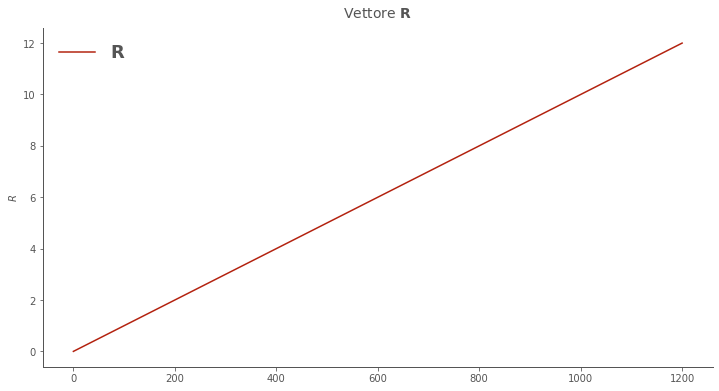
\includegraphics{vettorer.png}
        \caption{Vettore $\mathbf{R}$.}
        \label{fig:vettorer}
    \end{figure}

    
    \hypertarget{valori-noti}{%
\section{Valori noti}\label{valori-noti}}

    Si crea un vettore \(\mathbf{k_t}_{1\times \omega}\) di tutti i \(k\)
nuovi casi per giorno da \(t=0\) fino a oggi \(t=\omega\) (figura
\(\ref{fig:kt}\)). I dati italiani sono estratti dalla pubblicazione del
Dipartimento di Protezione Civile \cite{pcm_dpc_2020}.

    \[ t \in [0, \omega] \]

\[ \textrm{Nuovi casi al giorno } k_t \]

\[ \mathbf{k_t} = \begin{Bmatrix}
k_0 & k_1 & \cdots & k_\omega
\end{Bmatrix}_{1\times\omega} \]

    \[\mathbf{k_t} = \begin{Bmatrix} 124 & \cdots & 1284 \end{Bmatrix}_{1 \times 76}\]

    
    \[| \mathbf{k_t} | = 76\]

    
    
    \begin{figure}
    \centering
        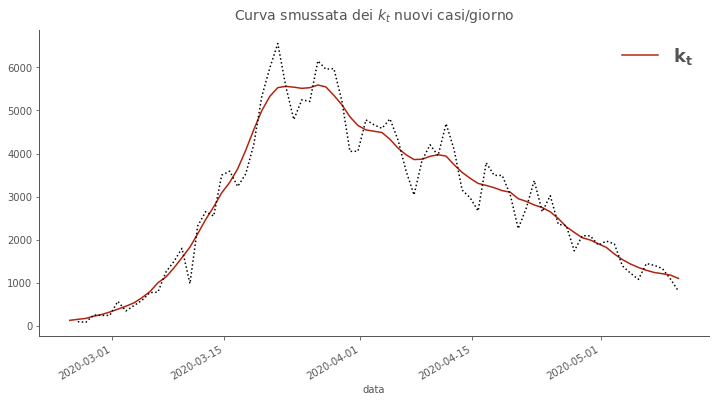
\includegraphics{kt.png}
        \caption{Curva smussata con metodo media mobile gaussiana ($\sigma=2.5$) dei nuovi casi per giorno in Italia. I valori $k_t$ formano il vettore $\mathbf{k_t}_{1 \times \omega}$}
        \label{fig:kt}
    \end{figure}

    
    \hypertarget{pkr}{%
\section{P(k\textbar R)}\label{pkr}}

    Per risolvere \(P(k_t^*|R)\) si nota anzitutto che, data una \(\lambda\)
serie di possibili \(k\) nuovi casi

\begin{equation}\label{eq:poisson}
P(k|\lambda) = \mathscr{P}(k, \lambda) = \frac{\lambda^k \cdot e^{-\lambda}}{k!}
\end{equation}

ovvero, la probabilità \textbf{a posteriori} di avere \(k\) nuovi casi
dati \(\lambda\) possibili valori \(k\) è una distribuzione di Poisson
di \(k\) con parametro \(\lambda\).

Sapendo però che il valore di \(k\) è noto (tutti i valori di \(k^*\)
sono nel vettore \(\mathbf{k_t}\)) si può dire che

\begin{equation}\label{eq:likelihoods}
P(k^*|\lambda) \propto \mathscr{L}(\lambda|k^*)
\end{equation}

ovvero, la probabilità di \emph{aver avuto} \(k^*\) nuovi casi date
\(\lambda\) possibilità è proporzionale alla verosimiglianza delle
\(\lambda\) possibilità noto \(k^*\).

Dalla letteratura, è nota la relazione tra \(\lambda\), \(k_t\) ed
\(R_t\):

\begin{equation}\label{eq:lambda}
\lambda = k_t \cdot \exp{\big[ \gamma (R_t - 1) \big]}
\end{equation}

Grazie a questa relazione è possibile dire che

\begin{equation}\label{eq:pkr}
P(k_t^*|R) = P(k_t^*|\lambda)
\end{equation}

e costruire una matrice \(\Lambda\) di \(\omega-1\) colonne (perché il
primo giorno è di outcome) e \(1201\) righe contenente per ogni giorno
\(t\) tutti i possibili valori di \(\lambda\) dati i possibili \(1201\)
valori di \(R\) (tabella \(\ref{tab:lambda}\) e figura
\(\ref{fig:lambda}\)).

    \begin{equation}\label{eq:matricelambda}
\Lambda = \mathbf{k_t} \cdot \exp\left[ \gamma ( \mathbf{R}^{T} - 1) \right], \; t=\left[ 0,\omega \right)
\end{equation}

\[ \Lambda = \begin{Bmatrix}
k_0 \cdot e^{\gamma (R_{min} - 1) } & \cdots  & k_{n-1} \cdot e^{\gamma (R_{min} - 1) } \\ 
\vdots & \vdots & \vdots \\ 
k_0 \cdot e^{\gamma (R_{max} - 1) } & \cdots  &  k_{n-1} \cdot e^{\gamma (R_{max} - 1) }  
\end{Bmatrix}_{1201 \times \omega-1} \]

    
\begin{table}
  \begin{center}
    \caption{Estratto di matrice $\Lambda$: $1201 \times 75$}
    \label{tab:lambda}
    \begin{tabular}{c|c|c|c|c|c|c|}
          & 2020-02-24 & 
          2020-02-25 &
          2020-02-26 &
          $\cdots$ & 
          2020-05-08 & 
          2020-05-09 \\
        \toprule
        $R=0.00$ & 108.52 & 128.65 & 147.90 & $\cdots$ & 1119.35 & 1119.35 \\
        \midrule
        $R=0.01$ & 108.67 & 128.82 & 148.10 & $\cdots$ & 1120.84 & 1120.84 \\
        \midrule
        $\vdots$ & $\vdots$ & $\vdots$ & $\vdots$ & $\vdots$ & $\vdots$ & $\vdots$ \\
        \midrule
        $R=11.99$ & 536.79 & 636.36 & 731.60 & $\cdots$ & 5536.77 & 5536.77 \\
        \midrule
        $R=12.00$ & 537.51 & 637.21 & 732.57 & $\cdots$ & 5544.16 & 5544.16 \\
        \bottomrule
    \end{tabular}
  \end{center}
\end{table}
        

    
    
    \begin{figure}
    \centering
        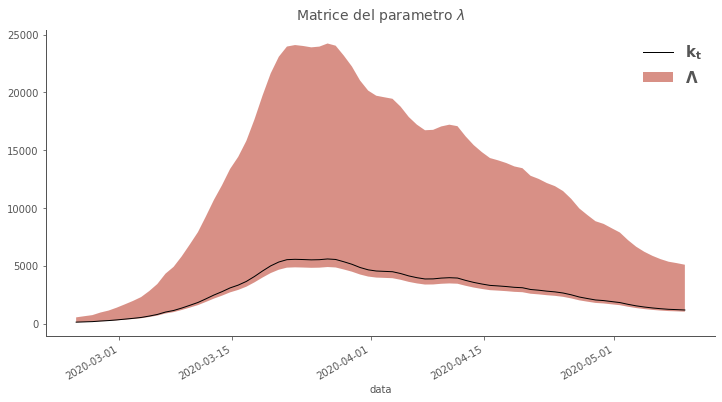
\includegraphics{lambda.png}
        \caption{Valori del parametro $\lambda$, ovvero matrice $\Lambda_{1201 \times \omega-1}$ sulla serie temporale. Per ogni giorno i valori $\lambda$ rappresentano tutti i possibili valori di $k_t$ dato il range di $R$ definito dal vettore $\mathbf{R} \in [R_{min},R_{max}]$.}
        \label{fig:lambda}
    \end{figure}

    
    Noti i valori della matrice \(\Lambda\) si può dunque applicare la
distribuzione di Poisson al vettore \(\mathbf{k_t}\) parametrizzata su
\(R\) con \(t \in (0,\omega]\) e ottenere così la matrice
\(\mathbf{P\big(k_t^* \;\big|\; R\big)}\) di tutte le verosimiglianze
dei possibili \(1201\) valori di \(R\) dati gli \(\omega-1\) valori di
\(k_t^*\) (figura \(\ref{fig:likelihoods}\) e tabella
\(\ref{tab:likelihoods}\)):

    \begin{equation}\label{eq:matricepkr}
P\big( \mathbf{k_t^*} \; \big| \; \Lambda \big)
= \mathscr{P} \big( \mathbf{k_t^*}, \Lambda \big) = 
\frac{\Lambda^{\mathbf{k_t^*}} \cdot e^{-\Lambda}}{\mathbf{k_t^*}!} = \\
= \mathbf{P\big( k_t^* \;\big|\; R \big)}_{1201 \times \omega-1}
\end{equation}

    
\begin{table}
  \begin{center}
    \caption{Estratto di matrice $\mathbf{P\big( k_t^* \;\big|\; R \big)}$ (valori normalizzati): $1201 \times 75$}
    \label{tab:likelihoods}
    \begin{tabular}{c|c|c|c|c|c|c|}
          & 2020-02-25 & 
          2020-02-26 &
          2020-02-27 &
          $\cdots$ & 
          2020-05-08 & 
          2020-05-09 \\
        \toprule
        $R=0.00$ & 1.40e-05 & 2.19e-05 & 1.25e-09 & $\cdots$ & 3.58e-07 & 1.82e-07 \\
        \midrule
        $R=0.01$ & 1.47e-05 & 2.31e-05 & 1.38e-09 & $\cdots$ & 4.43e-07 & 2.27e-07 \\
        \midrule
        $\vdots$ & $\vdots$ & $\vdots$ & $\vdots$ & $\vdots$ & $\vdots$ & $\vdots$ \\
        \midrule
        $R=11.99$ & 1.62e-89 & 1.52e-108 & 1.10e-109 & $\cdots$ & 0.00e+00 & 0.00e+00 \\
        \midrule
        $R=12.00$ & 9.64e-90 & 8.12e-109 & 5.56e-110 & $\cdots$ & 0.00e+00 & 0.00e+00 \\
        \bottomrule
    \end{tabular}
  \end{center}
\end{table}
        

    
    
    \begin{figure}
    \centering
        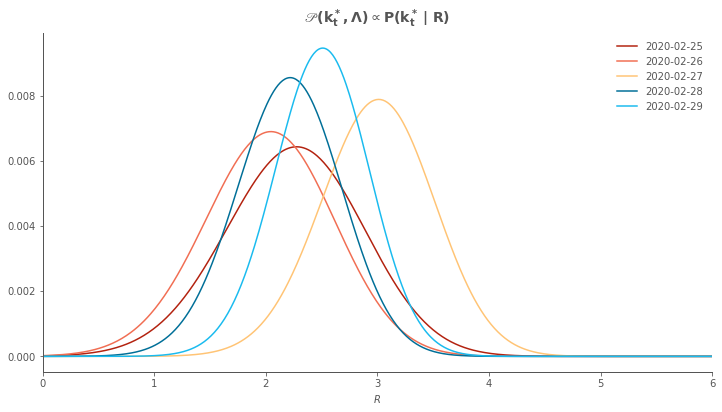
\includegraphics{likelihoods.png}
        \caption{Verosimiglianze $\mathbf{P( k_t^* \;|\; R )}$ dei primi 5 giorni di dati registrati in Italia. Valori normalizzati. Nella $\eqref{eq:formula1}$ non servirà normalizzare le verosimiglianze perché il denonimatore stesso ha funzione di normalizzazione. Si nota come ogni giorno diminuisca la deviazione standard e dunque si guadagni progressivamente in confidenza.}
        \label{fig:likelihoods}
    \end{figure}

    
    \hypertarget{pr}{%
\section{P(R)}\label{pr}}

    La probabilità \textbf{a priori} dei possibili valori \(R\) può essere
interpretata come una ditribuzione normale (Gaussiana) avente media
\(\mu = R\) e deviazione standard \(\sigma\) che può essere stimata a
\(0.25\).

Si può dunque creare una matrice \(\mathbf{P(R)}\) di
\(1201 \times 1201\) i cui elementi \(P(n)_m\) di riga \(n\) e colonna
\(m\) sono la probabilità di \(R=n\) con \(\mu=m\) (tabella
\(\ref{tab:pr}\), figure \(\ref{fig:pr1}\) e \(\ref{fig:pr2}\)):

    \begin{equation}\label{eq:pr}
\mathbf{P(R)} = \mathbf{\mathscr{N}(R,\sigma)} = \\
= 
\begin{Bmatrix}
P(0)_{0} & \cdots & P(0)_{6} & \cdots  & P(0)_{12} \\ 
\vdots & \ddots & \vdots & & \vdots \\
P(6)_{0} & \cdots & P(6)_{6} & \cdots & P(6)_{12} \\ 
\vdots & & \vdots & \ddots & \vdots \\
P(12)_{0} & \cdots & P(12)_{6} & \cdots & P(12)_{12}
\end{Bmatrix}_{1201 \times 1201}
\end{equation}

    
\begin{table}
  \begin{center}
    \caption{Estratto di matrice $\mathbf{P(R)}$: $1201 \times 1201$}
    \label{tab:pr}
    \begin{tabular}{c|c|c|c|c|c|c|}
          & $\mu=0.00$ &$\mu=0.01$ & $\mu=0.02$ & $\cdots$ & $\mu=11.99$ & $\mu=12.00$ \\
        \toprule
        $R=0.00$ & 3.14e-02 & 3.04e-02 & 2.95e-02 & $\cdots$ & 0.00e+00 & 0.00e+00 \\
        \midrule
        $R=0.01$ & 3.14e-02 & 3.05e-02 & 2.95e-02 & $\cdots$ & 0.00e+00 & 0.00e+00 \\
        \midrule
        $\vdots$ & $\vdots$ & $\vdots$ & $\vdots$ & $\vdots$ & $\vdots$ & $\vdots$ \\
        \midrule
        $R=11.99$ & 0.00e+00 & 0.00e+00 & 0.00e+00 & $\cdots$ & 3.05e-02 & 3.14e-02 \\
        \midrule
        $R=12.00$ & 0.00e+00 & 0.00e+00 & 0.00e+00 & $\cdots$ & 3.04e-02 & 3.14e-02 \\
        \bottomrule
    \end{tabular}
  \end{center}
\end{table}
        

    
    
    \begin{figure}
    \centering
        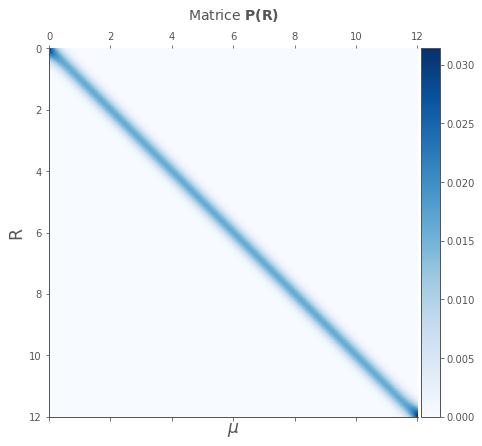
\includegraphics{pr1.png}
        \caption{Matrice $\mathbf{P(R)}$. Il colore indica la distribuzione di probabilità. Essendo gaussiana, è concentrata intorno a $\mu$ ovvero sulla diagonale della matrice.}
        \label{fig:pr1}
    \end{figure}

    
    
    \begin{figure}
    \centering
        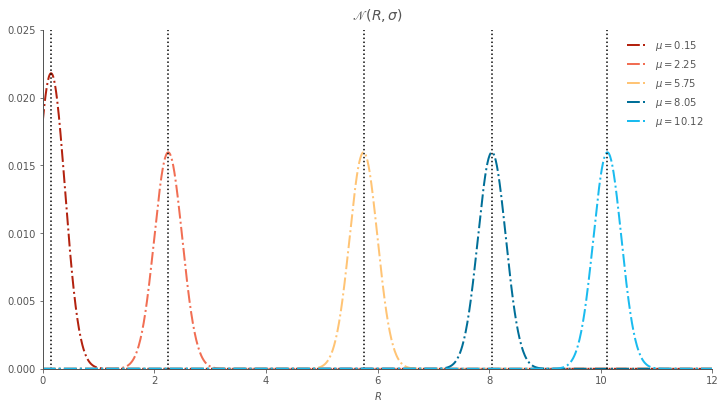
\includegraphics{pr2.png}
        \caption{Distribuzione gaussiana di $P(R)$ con $\sigma=0.25$.}
        \label{fig:pr2}
    \end{figure}

    
    \hypertarget{prk}{%
\section{P(R\textbar k)}\label{prk}}

    È dunque possibile ora creare una matrice vuota
\(\mathbf{P\big(R_t \;\big|\; k_t^*\big)}\) di \(1201 \times \omega\) i
cui elementi \(P(R_n)_m\) di riga \(n\) e colonna \(m\) saranno i valori
della probabilità di \(R=m\) al tempo \(t=n\) (tabella
\(\ref{tab:prkempty}\)).

    \begin{equation}\label{eq:matriceprk}
\mathbf{P\big(R_t \;\big|\; k_t^*\big)} = 
\begin{Bmatrix}
P(R_0)_{0} &  P(R_1)_{0} & \cdots  & P(R_\omega)_{0} \\ 
\vdots & \vdots & & \vdots \\
P(R_0)_{6} &  P(R_1)_{6} & \cdots & P(R_\omega)_{6} \\ 
\vdots & \vdots &  & \vdots \\
P(R_0)_{12} & P(R_1)_{12} & \cdots & P(R_\omega)_{12}
\end{Bmatrix}_{1201 \times \omega}
\end{equation}

    Non avendo alcuna informazione precedente a \(t=0\), si imposta la
probabilità iniziale della prima colonna
\(\mathbf{P\big(R_0 \;\big|\; k_0^*\big)}\) ovvero degli elementi
\(P(R_0)_m\) come costante in modo che \(\sum P(R_0)_m = 1\):

    \[P(R_0)_{m} = \frac{1}{ | \mathbf{R} | } = \frac{1}{1201} = 8.33e-04\]

    
    
\begin{table}
  \begin{center}
    \caption{Estratto di matrice vuota $\mathbf{P(R_t|k_t^*)}$: $1201 \times 76$}
    \label{tab:prkempty}
    \begin{tabular}{c|c|c|c|c|c|c|}
          & 2020-02-24 & 
          2020-02-25 &
          2020-02-26 &
          $\cdots$ & 
          2020-05-08 & 
          2020-05-09 \\
        \toprule
        $R=0.00$ & 8.33e-04 & nan & nan & $\cdots$ & nan & nan \\
        \midrule
        $R=0.01$ & 8.33e-04 & nan & nan & $\cdots$ & nan & nan \\
        \midrule
        $\vdots$ & $\vdots$ & $\vdots$ & $\vdots$ & $\vdots$ & $\vdots$ & $\vdots$ \\
        \midrule
        $R=11.99$ & 8.33e-04 & nan & nan & $\cdots$ & nan & nan \\
        \midrule
        $R=12.00$ & 8.33e-04 & nan & nan & $\cdots$ & nan & nan \\
        \bottomrule
    \end{tabular}
  \end{center}
\end{table}
        

    
    Per ogni giorno \(t \in (0, \omega]\) si calcola la probabilità di
\(R_t\) basata sulla distribuzione normale del giorno precedente \(t-1\)

    \begin{equation}\label{eq:prgiorno}
\begin{gathered}
\mathbf{P(R_t)_m} = \mathbf{P(R)}_{1201 \times 1201} \cdot \mathbf{P(R_{t-1})_m} = \\ %
= \begin{Bmatrix}
P(0)_{0} & \cdots & P(0)_{12} \\ 
\vdots & \ddots & \vdots \\
P(12)_{0} & \cdots & P(12)_{12}
\end{Bmatrix}_{1201 \times 1201}
\cdot
\begin{Bmatrix}
P(R_{t-1})_0  \\
\vdots \\ 
P(R_{t-1})_{12}
\end{Bmatrix}_{1201 \times 1} = \\ %
= \begin{Bmatrix}
P(R_{t})_0 \\
\vdots \\ 
P(R_{t})_{12}
\end{Bmatrix}_{1201 \times 1}
\end{gathered}
\end{equation}

    e si moltiplica per \(\mathbf{P(k_t^*|R)}\) calcolato in precedenza,
ottenendo così il numeratore della funzione \(\eqref{eq:formula1}\):

\begin{equation}\label{eq:numeratoreok}
\mathbf{P(k_t^*|R)} \cdot \mathbf{P(R_t)_m}
\end{equation}

Il denominatore \(P(k_t^*)\) è la sommatoria dei numeratori precedenti:

    \begin{equation}\label{eq:denominatoreok}
P(k_t^*) = \sum_{i=0}^{t} \bigg( \mathbf{P(k_i^*|R)} \cdot \mathbf{P(R_i)_m} \bigg)
\end{equation}

    ottenendo dunque per ogni giorno \(t\) la probabilità (tabella
\(\ref{tab:prkfull}\) e figura \(\ref{fig:prk}\))

\begin{equation}\label{eq:finale}
\mathbf{P(R_t|k_t^*)} = 
\left\{
\frac{ \mathbf{P(k_t^*|R)} \cdot \mathbf{P(R_t)_m} }{ 
\sum_{i=0}^{t} \bigg( \mathbf{P(k_i^*|R)} \cdot \mathbf{P(R_i)_m} \bigg)
}
\right\}_{1201 \times \omega}
\end{equation}

    
\begin{table}
  \begin{center}
    \caption{Estratto di matrice finale $\mathbf{P(R_t|k_t^*)}$: $1201 \times 76$}
    \label{tab:prkfull}
    \begin{tabular}{c|c|c|c|c|c|c|}
          & 2020-02-24 & 
          2020-02-25 &
          2020-02-26 &
          $\cdots$ & 
          2020-05-08 & 
          2020-05-09 \\
        \toprule
        $R=0.00$ & 8.33e-04 & 9.82e-06 & 1.45e-07 & $\cdots$ & 1.18e-08 & 1.87e-09 \\
        \midrule
        $R=0.01$ & 8.33e-04 & 1.06e-05 & 1.61e-07 & $\cdots$ & 1.59e-08 & 2.57e-09 \\
        \midrule
        $\vdots$ & $\vdots$ & $\vdots$ & $\vdots$ & $\vdots$ & $\vdots$ & $\vdots$ \\
        \midrule
        $R=11.99$ & 8.33e-04 & 1.17e-89 & 2.59e-171 & $\cdots$ & 0.00e+00 & 0.00e+00 \\
        \midrule
        $R=12.00$ & 8.33e-04 & 6.77e-90 & 9.84e-172 & $\cdots$ & 0.00e+00 & 0.00e+00 \\
        \bottomrule
    \end{tabular}
  \end{center}
\end{table}
        

    
    
    \begin{figure}
    \centering
        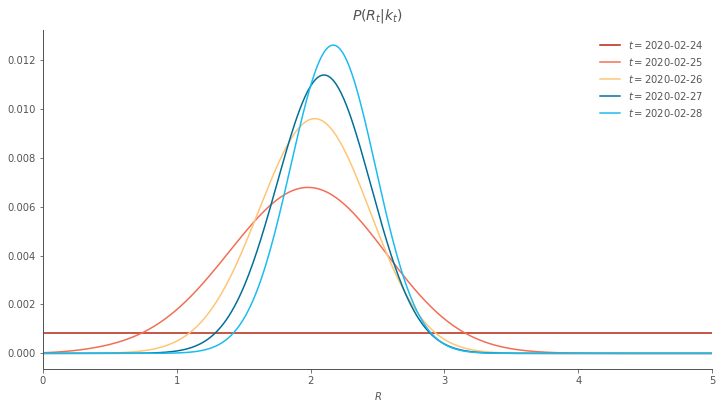
\includegraphics{prk.png}
        \caption{Ditribuzione di probabilità $P(R_t|k_t)$ dei primi 5 giorni di dati in Italia. Si nota come nel primo giorno, non avendo alcuna informazione la probabilità è equamente distribuita e successivamente ogni giorno diminuisca la deviazione standard e dunque si guadagni progressivamente in confidenza sul valore di $R_t$.}
        \label{fig:prk}
    \end{figure}

    
    Per ogni tempo \(t\) ovvero per ogni colonna della matrice
\(\mathbf{{P(R_t|k_t^*)}}\) \(\eqref{eq:finale}\) si calcola il valore
massimo ovvero il valore di \(R_t\) maggiormente probabile e
l'intervallo di confidenza, che può essere stabilito al 90\%, ottenendo
la tabella di valori di \(R_t\) per ogni giorno \(t\) (tabella
\(\ref{tab:rt}\) e figura \(\ref{fig:rtbars}\)) e produrre un grafico
dell'intera serie temporale (figura \(\ref{fig:rtitalia}\)).

    
    \begin{figure}
    \centering
        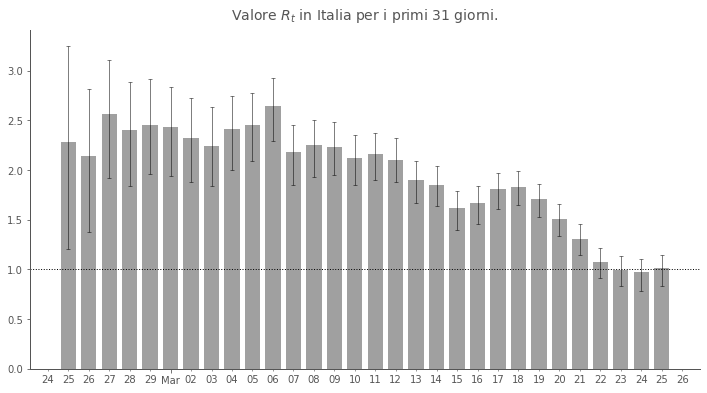
\includegraphics{rtbars.png}
        \caption{Valore $R_t$ in Italia per i primi 31 giorni con itervallo di confidenza al 90\%.Il primo giorno, non avendo informazioni sui precedenti, serve solo da precedente.}
        \label{fig:rtbars}
    \end{figure}

    
    
\begin{table}
  \begin{center}
    \caption{Estratto di tabella dei valori $R_t$: $76 \times 3$}
    \label{tab:rt}
    \begin{tabular}{c|c|c|c|}
        & Lo 90 & max & Hi 90 \\
        \toprule
        2020-02-24 & 0.00 & 0.00 & 10.81 \\
        \midrule
        2020-02-25 & 1.21 & 2.28 & 3.25 \\
        \midrule
        $\vdots$ & $\vdots$ & $\vdots$ & $\vdots$ \\
        \midrule
        2020-05-08 & 0.65 & 0.95 & 1.22 \\
        \midrule
        2020-05-09 & 0.70 & 1.00 & 1.27 \\
        \bottomrule
    \end{tabular}
  \end{center}
\end{table}
        

    
    
    \begin{figure}
    \centering
        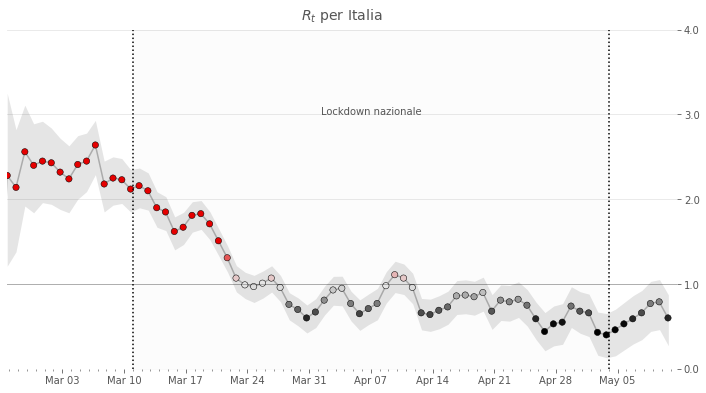
\includegraphics{rtitalia.png}
        \caption{Valori di $R_t$ in Italia con intervallo di confidenza al 90\%.}
        \label{fig:rtitalia}
    \end{figure}

    
    \hypertarget{conclusioni}{%
\section{Conclusioni}\label{conclusioni}}

    È dunque possibile stimare il valore del numero di riproduzione
effettivo \(R_t\) in base al numero noto di nuovi casi giornalieri
\(k_t\) e al tempo seriale \(T_{serial}\) con metodo Bayesiano
\(P(R_t|k_t)\), utilizzando i risultati del giorno precedente come base
per il calcolo della probabilità a posteriori, scegliendo l'intervallo
di confidenza desiderato. È consigliabile smussare la curva dei nuovi
casi (con media mobile) per diminuire la variabilità dovuta errori e
correzioni nella collezione giornaliera dei dati.

    \hypertarget{codice-python}{%
\section{Codice Python}\label{codice-python}}

    Si fornisce di seguito un esempio di codice \texttt{Python} per
l'esecuzione del metodo illustrato per il calcolo di \(R_t\) in Italia,
adattato dalla versione di Kevin Systrom \cite{k-sys}.

    \begin{Shaded}
\begin{Highlighting}[]
\ImportTok{import}\NormalTok{ numpy }\ImportTok{as}\NormalTok{ np}
\ImportTok{import}\NormalTok{ pandas }\ImportTok{as}\NormalTok{ pd}
\ImportTok{import}\NormalTok{ scipy.stats }\ImportTok{as}\NormalTok{ sps}

\CommentTok{\# DEF: Calcolo nuovi casi e media mobile}
\KeywordTok{def}\NormalTok{ smooth(y, std}\OperatorTok{=}\DecValTok{2}\NormalTok{):}
\NormalTok{    dy }\OperatorTok{=}\NormalTok{ y.diff()}
\NormalTok{    dy\_smoothed }\OperatorTok{=}\NormalTok{ dy.rolling(}\DecValTok{7}\NormalTok{,}
\NormalTok{            win\_type}\OperatorTok{=}\StringTok{"gaussian"}\NormalTok{,}
\NormalTok{            min\_periods}\OperatorTok{=}\DecValTok{1}\NormalTok{,}
\NormalTok{            center}\OperatorTok{=}\VariableTok{True}\NormalTok{).mean(std}\OperatorTok{=}\NormalTok{std).}\BuiltInTok{round}\NormalTok{()}
    \ControlFlowTok{return}\NormalTok{ dy\_smoothed, dy}

\CommentTok{\# DEF: Estrazione intervallo di confidenza}
\KeywordTok{def}\NormalTok{ highest\_density\_interval(pmf, p}\OperatorTok{=}\FloatTok{.9}\NormalTok{):}
    \ControlFlowTok{if}\NormalTok{(}\BuiltInTok{isinstance}\NormalTok{(pmf, pd.DataFrame)):}
        \ControlFlowTok{return}\NormalTok{ pd.DataFrame(}
\NormalTok{            [highest\_density\_interval(}
\NormalTok{                pmf[col], p}\OperatorTok{=}\NormalTok{p}
\NormalTok{            ) }\ControlFlowTok{for}\NormalTok{ col }\KeywordTok{in}\NormalTok{ pmf],}
\NormalTok{            index}\OperatorTok{=}\NormalTok{pmf.columns)}
    
\NormalTok{    cumsum }\OperatorTok{=}\NormalTok{ np.cumsum(pmf.values)}
\NormalTok{    total\_p }\OperatorTok{=}\NormalTok{ cumsum }\OperatorTok{{-}}\NormalTok{ cumsum[:, }\VariableTok{None}\NormalTok{]}
\NormalTok{    lows, highs }\OperatorTok{=}\NormalTok{ (total\_p }\OperatorTok{\textgreater{}}\NormalTok{ p).nonzero()}
\NormalTok{    best }\OperatorTok{=}\NormalTok{ (highs }\OperatorTok{{-}}\NormalTok{ lows).argmin()}
\NormalTok{    low }\OperatorTok{=}\NormalTok{ pmf.index[lows[best]]}
\NormalTok{    high }\OperatorTok{=}\NormalTok{ pmf.index[highs[best]]}
    
    \ControlFlowTok{return}\NormalTok{ pd.Series(}
\NormalTok{        [low, high],}
\NormalTok{        index}\OperatorTok{=}\NormalTok{[}
            \SpecialStringTok{f"Low\_}\SpecialCharTok{\{p}\OperatorTok{*}\DecValTok{100}\SpecialCharTok{:.0f\}}\SpecialStringTok{"}\NormalTok{,}
            \SpecialStringTok{f"High\_}\SpecialCharTok{\{p}\OperatorTok{*}\DecValTok{100}\SpecialCharTok{:.0f\}}\SpecialStringTok{"}\NormalTok{])}

\CommentTok{\#\#\#\#\#\#\#\#\#\#\# CALCOLO \#\#\#\#\#\#\#\#\#\#\#}

\CommentTok{\# Intervallo seriale e gamma}
\NormalTok{T\_serial }\OperatorTok{=} \FloatTok{7.5}
\NormalTok{gamma }\OperatorTok{=} \DecValTok{1} \OperatorTok{/}\NormalTok{ T\_serial}

\CommentTok{\# Vettori R}
\NormalTok{Rt\_min }\OperatorTok{=} \DecValTok{0}
\NormalTok{Rt\_max }\OperatorTok{=} \DecValTok{12}
\NormalTok{Rt\_bra }\OperatorTok{=}\NormalTok{ np.linspace(Rt\_min, Rt\_max, Rt\_max}\OperatorTok{*}\DecValTok{100}\OperatorTok{+}\DecValTok{1}\NormalTok{)}
\NormalTok{Rt\_ket }\OperatorTok{=}\NormalTok{ Rt\_bra[:, }\VariableTok{None}\NormalTok{]}

\CommentTok{\# Caricamento dati}
\NormalTok{url\_base }\OperatorTok{=} \StringTok{"https://raw.githubusercontent.com/"}
\NormalTok{url\_repo }\OperatorTok{=} \StringTok{"pcm{-}dpc/COVID{-}19/master/dati{-}andamento{-}nazionale/"}
\NormalTok{url\_file }\OperatorTok{=} \StringTok{"dpc{-}covid19{-}ita{-}andamento{-}nazionale.csv"} 
\NormalTok{url\_ita }\OperatorTok{=}\NormalTok{ url\_base }\OperatorTok{+}\NormalTok{ url\_repo }\OperatorTok{+}\NormalTok{ url\_file}
\NormalTok{ita }\OperatorTok{=}\NormalTok{ pd.read\_csv(}
\NormalTok{    url\_ita,}
\NormalTok{    usecols}\OperatorTok{=}\NormalTok{[}\StringTok{"data"}\NormalTok{, }\StringTok{"totale\_casi"}\NormalTok{],}
\NormalTok{    parse\_dates}\OperatorTok{=}\NormalTok{[}\StringTok{"data"}\NormalTok{],}
\NormalTok{    index\_col}\OperatorTok{=}\NormalTok{[}\StringTok{"data"}\NormalTok{],}
\NormalTok{    squeeze}\OperatorTok{=}\VariableTok{True}\NormalTok{).sort\_index()}

\CommentTok{\# Calcolo nuovi casi e media mobile}
\NormalTok{k\_bra, orig }\OperatorTok{=}\NormalTok{ smooth(ita, std}\OperatorTok{=}\FloatTok{2.5}\NormalTok{)}

\CommentTok{\# Matrice lambda}
\NormalTok{lam }\OperatorTok{=}\NormalTok{ k\_bra[:}\OperatorTok{{-}}\DecValTok{1}\NormalTok{].values }\OperatorTok{*}\NormalTok{ np.exp(gamma }\OperatorTok{*}\NormalTok{ (Rt\_ket }\OperatorTok{{-}} \DecValTok{1}\NormalTok{))}

\CommentTok{\# Matrice verosimiglianze P(k*|R)}
\NormalTok{likelihoods }\OperatorTok{=}\NormalTok{ pd.DataFrame(}
\NormalTok{    data }\OperatorTok{=}\NormalTok{ sps.poisson.pmf(k\_bra[}\DecValTok{1}\NormalTok{:].values, lam),}
\NormalTok{    index }\OperatorTok{=}\NormalTok{ Rt\_bra,}
\NormalTok{    columns }\OperatorTok{=}\NormalTok{ k\_bra.index[}\DecValTok{1}\NormalTok{:])}

\CommentTok{\# Matrice P(R)}
\NormalTok{sigma }\OperatorTok{=} \FloatTok{.25}
\NormalTok{process\_matrix }\OperatorTok{=}\NormalTok{ sps.norm(}
\NormalTok{    loc}\OperatorTok{=}\NormalTok{Rt\_bra,}
\NormalTok{    scale}\OperatorTok{=}\NormalTok{sigma}
\NormalTok{).pdf(Rt\_ket)}
\NormalTok{process\_matrix }\OperatorTok{/=}\NormalTok{ process\_matrix.}\BuiltInTok{sum}\NormalTok{(axis}\OperatorTok{=}\DecValTok{0}\NormalTok{)}

\CommentTok{\# Primo precedente della matrice P(R|k)}
\NormalTok{prior0 }\OperatorTok{=}\NormalTok{ np.ones\_like(Rt\_bra)}\OperatorTok{/}\BuiltInTok{len}\NormalTok{(Rt\_bra)}
\NormalTok{prior0 }\OperatorTok{/=}\NormalTok{ prior0.}\BuiltInTok{sum}\NormalTok{()}

\CommentTok{\# Matrice vuota P(R|k)}
\NormalTok{posteriors }\OperatorTok{=}\NormalTok{ pd.DataFrame(}
\NormalTok{    index}\OperatorTok{=}\NormalTok{Rt\_bra,}
\NormalTok{    columns}\OperatorTok{=}\NormalTok{k\_bra.index,}
\NormalTok{    data}\OperatorTok{=}\NormalTok{\{k\_bra.index[}\DecValTok{0}\NormalTok{]: prior0\}}
\NormalTok{)}

\CommentTok{\# Calcolo P(R|k*) giorno per giorno}
\ControlFlowTok{for}\NormalTok{ previous\_day, current\_day }\KeywordTok{in} \BuiltInTok{zip}\NormalTok{(k\_bra.index[:}\OperatorTok{{-}}\DecValTok{1}\NormalTok{], k\_bra.index[}\DecValTok{1}\NormalTok{:]):}
    \CommentTok{\# Calcolo del precedente P(R\_t) = P(R) * P(R\_(t{-}1))}
\NormalTok{    current\_prior }\OperatorTok{=}\NormalTok{ process\_matrix }\OperatorTok{@}\NormalTok{ posteriors[previous\_day]}
    \CommentTok{\# Calcolo numeratore P(k*|R)P(R\_t) [equazione (2)]}
\NormalTok{    numerator }\OperatorTok{=}\NormalTok{ likelihoods[current\_day] }\OperatorTok{*}\NormalTok{ current\_prior}
    \CommentTok{\# Calcolo denominatore P(k*) [equazione (2) e (3)]}
\NormalTok{    denominator }\OperatorTok{=}\NormalTok{ np.}\BuiltInTok{sum}\NormalTok{(numerator)}
    \CommentTok{\# Calcolo della probabilità a posteriori P(k*|R\_t) [equazione (2)]}
\NormalTok{    posteriors[current\_day] }\OperatorTok{=}\NormalTok{ numerator}\OperatorTok{/}\NormalTok{denominator}

\CommentTok{\# Estrazione valori per intervallo di confidenza p}
\NormalTok{hdis }\OperatorTok{=}\NormalTok{ highest\_density\_interval(posteriors, p}\OperatorTok{=}\FloatTok{.9}\NormalTok{)}

\CommentTok{\# Estrazione massima probabilità}
\NormalTok{most\_likely }\OperatorTok{=}\NormalTok{ posteriors.idxmax().rename(}\StringTok{"ML"}\NormalTok{)}

\CommentTok{\# Tabella valori di R in t}
\NormalTok{result }\OperatorTok{=}\NormalTok{ pd.concat([most\_likely, hdis], axis}\OperatorTok{=}\DecValTok{1}\NormalTok{)}
\end{Highlighting}
\end{Shaded}


    % Add a bibliography block to the postdoc
    
    
\bibliographystyle{IEEEtran}
\bibliography{IEEEabrv,articolo}

    
\end{document}
